\documentclass[a4paper,11pt]{article}

% ── Kodowanie i język ──
\usepackage[T1]{fontenc}
\usepackage[utf8]{inputenc}
\usepackage[polish]{babel}

% ── Marginesy ──
\usepackage[margin=2.5cm]{geometry}

% ── Matematyka ──
\usepackage{amsmath}
\usepackage{amssymb}
\usepackage{siunitx}
\sisetup{
    output-decimal-marker = {,},
    per-mode = symbol,
    range-phrase = { -- },
}

% ── Grafika i tabele ──
\usepackage{graphicx}
\usepackage{float}
\usepackage{booktabs}
\usepackage{array}
\usepackage{tabularx}
\usepackage{multirow}
\usepackage{caption}
\usepackage{subcaption}

% ── Kolory i linki ──
\usepackage[dvipsnames]{xcolor}
\usepackage{hyperref}
\hypersetup{
    colorlinks=true,
    linkcolor=NavyBlue,
    citecolor=NavyBlue,
    urlcolor=RoyalBlue,
}

% ── Listingi kodu ──
\usepackage{listings}
\lstset{
    language=C,
    basicstyle=\ttfamily\footnotesize,
    keywordstyle=\color{NavyBlue}\bfseries,
    commentstyle=\color{Gray}\itshape,
    stringstyle=\color{OliveGreen},
    numbers=left,
    numberstyle=\tiny\color{Gray},
    frame=single,
    breaklines=true,
    captionpos=b,
    tabsize=4,
    showstringspaces=false,
}

% ── Flowcharty / diagramy ──
\usepackage{tikz}
\usetikzlibrary{shapes.geometric, arrows.meta, positioning, calc, patterns, decorations.markings}

% ── Nagłówek / stopka ──
\usepackage{fancyhdr}
\pagestyle{fancy}
\fancyhf{}
\fancyhead[L]{\small Bezkontaktowy miernik odległości — Pulse-Phase Ranging}
\fancyhead[R]{\small Wygraj Indeks WETI 2026}
\fancyfoot[C]{\thepage}
\renewcommand{\headrulewidth}{0.4pt}

% ── Odstępy ──
\usepackage{setspace}
\onehalfspacing
\usepackage{parskip}

% ── Enumerate customization ──
\usepackage{enumitem}

% ══════════════════════════════════════════════════════════════
\begin{document}

% ── STRONA TYTUŁOWA ──────────────────────────────────────────
\begin{titlepage}
    \centering
    \vspace*{1.5cm}

    {\Large Ogólnopolski Konkurs Projektowy}\\[0.3cm]
    {\Large\textbf{,,Wygraj Indeks WETI'' --- edycja 2026}}\\[0.2cm]
    {\large Wydział Elektroniki, Telekomunikacji i~Informatyki\\
    Politechnika Gdańska}

    \vspace{1.5cm}

    {\Huge\bfseries Bezkontaktowy miernik odległości}\\[0.5cm]
    {\Large Metoda hybrydowa Pulse-Phase Ranging\\z~kompensacją temperatury}

    \vspace{1.5cm}

    % ── Schemat blokowy na stronie tytułowej ──
    \begin{tikzpicture}[
        block/.style={rectangle, draw, fill=NavyBlue!10, minimum width=2.2cm, minimum height=1cm, align=center, font=\small},
        arr/.style={->, >=Stealth, thick},
        scale=0.9, transform shape
    ]
        \node[block] (psu) {Zasilanie\\5V$\to$3{,}3V};
        \node[block, right=1.5cm of psu] (tx) {Nadajnik\\TX 40\,kHz};
        \node[block, right=1.5cm of tx] (rx) {Odbiornik\\RX + Filtr};
        \node[block, right=1.5cm of rx] (mcu) {ATtiny1616\\MCU};
        \node[block, below=1.0cm of tx] (temp) {Termistor\\NTC};

        % Zasilanie -> Nadajnik
        \draw[arr] (psu) -- (tx);
        % Zasilanie -> MCU (górą)
        \draw[arr] (psu.north) -- ++(0,0.5) -| (mcu.north);
        % MCU -> TX burst (górą, niebieski)
        \draw[arr, NavyBlue] (mcu.north east) ++(0,0.2) -- ++(0,0.8) -| node[above, pos=0.25, font=\scriptsize] {Burst 40\,kHz} (tx.north);
        % MCU -> RX sterowanie (PWM)
        \draw[arr] (mcu.west) -- node[below, font=\scriptsize] {PWM} (rx.east);
        % RX -> MCU echo (dołem, czerwony)
        \draw[arr, red] (rx.south east) -- ++(0,-0.5) -| node[below, pos=0.3, font=\scriptsize, text=red] {Echo (ADC)} (mcu.south);
        % Termistor -> MCU
        \draw[arr, gray] (temp.east) -| (mcu.south west);
        \node[gray, font=\scriptsize] at ($(temp.east)+(1.5,-0.3)$) {NTC (ADC)};
        % Fala US
        \draw[arr, blue, thick, loosely dashed]
            (tx.south west) -- ++(0,-0.5) node[below, font=\scriptsize] {Fala US};
    \end{tikzpicture}

    \vfill

    {\large
    \begin{tabular}{rl}
        \textbf{Autor:}  & Kacper Popko \\
        \textbf{Szkoła:}  & II Liceum Ogólnokształcące im.\ ks.\ Anny z~Sapiehów \\
                          & Jabłonowskiej w~Białymstoku \\
        \textbf{E-mail:}  & kacper@kajpa.pl \\
        \textbf{Data:}    & Marzec 2026 \\
    \end{tabular}
    }

    \vspace{1cm}
\end{titlepage}

% ── SPIS TREŚCI ──────────────────────────────────────────────
\tableofcontents
\newpage

% ══════════════════════════════════════════════════════════════
% SEKCJA 1: WSTĘP
% ══════════════════════════════════════════════════════════════
\section{Wstęp}
\label{sec:wstep}

Celem projektu jest opracowanie bezkontaktowego miernika odległości spełniającego
wymagania konkursu ,,Wygraj Indeks WETI 2026''. Urządzenie umożliwia pomiar
odległości w~zakresie \SIrange{10}{50}{\centi\metre} od obiektu (arkusz kartonu
$20 \times 20$~\si{\centi\metre}) przy zasilaniu napięciem \SI{5}{\volt}.

Jako metodę pomiarową wybrano \textbf{hybrydową technikę Pulse-Phase Ranging},
łączącą pomiar czasu przelotu impulsu ultradźwiękowego (ToF) z~pomiarem
przesunięcia fazowego sygnału echa. Podejście to pozwala uzyskać rozdzielczość
rzędu \SI{0,1}{\milli\metre} przy jednoczesnym zachowaniu jednoznaczności pomiaru
w~całym wymaganym zakresie --- łączy zalety obu metod, eliminując ich indywidualne
ograniczenia.

Projekt kładzie szczególny nacisk na trzy aspekty optymalizacyjne wynikające
z~kryteriów oceny konkursowej: minimalizację błędu średniokwadratowego (RMSE)
poprzez zaawansowany algorytm pomiaru fazowego, redukcję poboru mocy dzięki
agresywnej polityce uśpienia mikrokontrolera oraz minimalizację kosztu
komponentów przy zachowaniu wysokiej jakości toru pomiarowego.

\subsection{Wymagania konkursowe}

\begin{table}[H]
    \centering
    \caption{Podsumowanie wymagań konkursowych i~kryteriów oceny}
    \label{tab:wymagania}
    \begin{tabular}{lll}
        \toprule
        \textbf{Parametr}       & \textbf{Wartość / Wzór} & \textbf{Max pkt} \\
        \midrule
        Napięcie zasilania      & \SI{5}{\volt}  & --- \\
        Zakres pomiaru          & \SI{10}{\centi\metre} -- \SI{50}{\centi\metre} & --- \\
        Wykrywany obiekt        & Karton $20 \times 20$~\si{\centi\metre} & --- \\
        Błąd RMSE               & Im mniejszy, tym lepiej & 100 \\
        Pobór mocy              & $100 / P_{[\si{\milli\watt}]}$ & 50 \\
        Koszt elementów         & $50 \cdot 50 / C_{[\text{PLN}]}$ & 50 \\
        Jakość projektu         & Uznaniowo (komisja) & 100 \\
        \midrule
        \textbf{Łącznie}        & & \textbf{300} \\
        \bottomrule
    \end{tabular}
\end{table}

\subsection{Uzasadnienie wyboru metody pomiarowej}

Przed przystąpieniem do projektowania przeanalizowano cztery główne metody
bezkontaktowego pomiaru odległości pod kątem ich realizowalności na platformie
ATtiny1616 oraz potencjału punktacyjnego w~konkursie.

\begin{table}[H]
    \centering
    \caption{Analiza porównawcza rozważanych metod pomiaru}
    \label{tab:porownanie_metod}
    \begin{tabularx}{\textwidth}{lcccX}
        \toprule
        \textbf{Metoda} & \textbf{RMSE} & \textbf{Koszt} & \textbf{Złożoność} & \textbf{Uwagi} \\
        \midrule
        Prosty ToF (US)
            & ${\sim}\SI{3}{\milli\metre}$
            & Niski
            & Niska
            & Rozdzielczość ograniczona przez czas narastania obwiedni przetwornika rezonansowego; brak możliwości sub-milimetrowej dokładności \\[6pt]
        \textbf{Pulse-Phase (US)}
            & ${\sim}\SI{0,5}{\milli\metre}$
            & \textbf{Niski}
            & Średnia
            & \textbf{Wybrany kompromis} --- gruby pomiar ToF eliminuje niejednoznaczność fazową, dokładny pomiar fazy daje sub-mm rozdzielczość \\[6pt]
        FMCW chirp (US)
            & ${<}\SI{0,5}{\milli\metre}$
            & Średni
            & Wysoka
            & Wymaga szerokopasmowych przetworników US (${\sim}\SI{30}{PLN}$/para) oraz FFT --- ATtiny1616 z~16\,KB Flash i~2\,KB RAM nie ma wystarczających zasobów \\[6pt]
        Triangulacja optyczna
            & ${\sim}\SI{1}{\milli\metre}$
            & Średni
            & Średnia
            & Wymaga precyzyjnej mechaniki mocowania LED/fotodiody; wrażliwość na oświetlenie otoczenia; trudna powtarzalność prototypu \\
        \bottomrule
    \end{tabularx}
\end{table}

Metoda Pulse-Phase Ranging została wybrana jako oferująca najlepszy stosunek
osiągalnej dokładności do złożoności implementacji. Kluczowe argumenty:

\begin{enumerate}[nosep]
    \item Wykorzystuje tanie przetworniki rezonansowe \SI{40}{\kilo\hertz} (koszt pary: ${\sim}\SI{6}{PLN}$).
    \item Algorytm Goertzela do wyznaczania fazy wymaga jedynie ${\sim}\SI{200}{\byte}$ RAM.
    \item Kompensacja temperatury termistorem NTC eliminuje dominujące źródło błędu systematycznego.
    \item Tryb uśpienia ATtiny1616 (Power-Down, $I_{DD} = \SI{0,1}{\micro\ampere}$) pozwala osiągnąć średni pobór mocy poniżej \SI{2}{\milli\watt}.
\end{enumerate}


% ══════════════════════════════════════════════════════════════
% SEKCJA 2: ZASADA DZIAŁANIA
% ══════════════════════════════════════════════════════════════
\section{Zasada działania metody Pulse-Phase Ranging}
\label{sec:zasada}

\subsection{Przegląd metody}

Metoda Pulse-Phase Ranging łączy dwa pomiary wykonywane w~jednym cyklu
pomiarowym: gruby pomiar czasu przelotu (ToF) oraz dokładny pomiar przesunięcia
fazowego echa. Takie podejście rozwiązuje fundamentalny problem pomiaru fazowego
--- niejednoznaczność co $\lambda/2$ --- przy jednoczesnym zachowaniu sub-milimetrowej
rozdzielczości.

Cykl pomiarowy składa się z~następujących etapów:
\begin{enumerate}[nosep]
    \item Odczyt temperatury z~termistora NTC (korekcja $v(T)$).
    \item Generacja burstu TX: $N = 8$ cykli sygnału \SI{40}{\kilo\hertz}.
    \item Detekcja początku echa --- pomiar gruby $t_{ToF}$ (timer TCB0).
    \item Próbkowanie sygnału echa w~oknie pomiarowym (ADC0, ${\sim}4$ cykle po ustabilizowaniu się obwiedni).
    \item Obliczenie fazy algorytmem Goertzela --- pomiar dokładny $\varphi$.
    \item Fuzja obu pomiarów i~filtracja wyniku.
    \item Transmisja wyniku przez USART.
    \item Przejście w~tryb Power-Down do następnego cyklu.
\end{enumerate}

\subsection{Faza 1 --- Pomiar gruby (Time-of-Flight)}
\label{sec:tof}

Mikrokontroler generuje burst $N = 8$ cykli sygnału prostokątnego o~częstotliwości
$f_0 = \SI{40}{\kilo\hertz}$ za pomocą timera TCA0 w~trybie PWM. Sygnał
steruje tranzystorem BC817-40, który pobudza nadajnik ultradźwiękowy.

Czas przelotu impulsu do obiektu i~z~powrotem:
\begin{equation}
    t_{ToF} = \frac{2D}{v(T)}
    \label{eq:tof}
\end{equation}

gdzie $D$ to odległość od obiektu, a~$v(T)$ to prędkość dźwięku zależna
od temperatury powietrza:
\begin{equation}
    v(T) = 331{,}3 + 0{,}606 \cdot T \quad [\si{\metre\per\second}]
    \label{eq:predkosc_dzwieku}
\end{equation}

Dla zakresu pomiarowego \SIrange{10}{50}{\centi\metre} przy $T = \SI{20}{\celsius}$
($v \approx \SI{343,5}{\metre\per\second}$):
\begin{equation}
    t_{ToF,min} = \frac{2 \cdot 0{,}10}{343{,}5} \approx \SI{0,58}{\milli\second}, \qquad
    t_{ToF,max} = \frac{2 \cdot 0{,}50}{343{,}5} \approx \SI{2,91}{\milli\second}
    \label{eq:tof_zakres}
\end{equation}

Timer TCB0 taktowany zegarem \SI{20}{\mega\hertz} daje rozdzielczość
czasową \SI{50}{\nano\second}, co odpowiada rozdzielczości odległości:
\begin{equation}
    \Delta D_{tick} = \frac{v(T)}{2 \cdot f_{clk}} = \frac{343{,}5}{2 \cdot 20 \times 10^6} \approx \SI{8,6}{\micro\metre} \text{ / takt}
    \label{eq:rozdzielczosc_tick}
\end{equation}

Jednak realna rozdzielczość pomiaru grubego jest ograniczona przez czas narastania
obwiedni sygnału echa. Przetworniki rezonansowe \SI{40}{\kilo\hertz} mają
dobroć $Q \approx 15$, co oznacza czas narastania obwiedni:
\begin{equation}
    \tau_{rise} \approx \frac{Q}{\pi f_0} = \frac{15}{\pi \cdot 40000} \approx \SI{0,12}{\milli\second}
    \label{eq:tau_rise}
\end{equation}

Niepewność momentu detekcji progu obwiedni przekłada się na praktyczną
rozdzielczość pomiaru grubego rzędu \SIrange{1}{3}{\milli\metre}. To wystarczy
do jednoznacznego wyznaczenia liczby $n$ półfal w~równaniu (\ref{eq:wynik}),
ponieważ $\lambda/2 \approx \SI{4,3}{\milli\metre}$.

\subsection{Faza 2 --- Pomiar dokładny (Phase Measurement)}
\label{sec:phase}

Po detekcji echa mikrokontroler otwiera okno pomiarowe i~próbkuje sygnał
echo za pomocą ADC0. Z~zebranych próbek obliczane jest przesunięcie fazowe
$\varphi$ między sygnałem nadawanym (referencyjnym) a~sygnałem echa.

Odległość wynikająca z~pomiaru fazowego:
\begin{equation}
    D_{fine} = \frac{\varphi}{2\pi} \cdot \frac{\lambda}{2}
    \label{eq:phase}
\end{equation}

gdzie $\lambda = v(T) / f_0$ to długość fali ultradźwiękowej. Przy
$T = \SI{20}{\celsius}$:
\begin{equation}
    \lambda = \frac{343{,}5}{40000} \approx \SI{8,59}{\milli\metre}, \qquad
    \frac{\lambda}{2} \approx \SI{4,29}{\milli\metre}
    \label{eq:lambda}
\end{equation}

Pomiar fazowy daje niejednoznaczność co $\lambda/2 \approx \SI{4,3}{\milli\metre}$,
którą rozwiązuje pomiar gruby ToF (sekcja \ref{sec:tof}).

Wynikowa odległość po fuzji obu pomiarów:
\begin{equation}
    \boxed{D = n \cdot \frac{\lambda}{2} + D_{fine}}
    \label{eq:wynik}
\end{equation}

gdzie $n = \left\lfloor D_{ToF} / (\lambda/2) + 0{,}5 \right\rfloor$ to liczba
całkowitych półfal wyznaczona z~pomiaru grubego.

\subsubsection{Rozdzielczość pomiaru fazowego}

Rozdzielczość pomiaru fazy zależy od rozdzielczości ADC i~stosunku sygnału
do szumu (SNR). Przy 10-bitowym ADC i~$K$ próbkach na cykl:
\begin{equation}
    \Delta\varphi_{min} \approx \frac{2\pi}{2^{10} \cdot \sqrt{K/2}} = \frac{2\pi}{1024 \cdot \sqrt{K/2}}
    \label{eq:phase_res}
\end{equation}

Dla $K = 4$ próbek na cykl ($f_s = 4 \cdot f_0 = \SI{160}{\kilo\hertz}$):
\begin{equation}
    \Delta\varphi_{min} \approx \frac{2\pi}{1024 \cdot \sqrt{2}} \approx \SI{4,34}{\milli\radian}
\end{equation}

Co odpowiada rozdzielczości odległości:
\begin{equation}
    \Delta D_{phase} = \frac{\Delta\varphi_{min}}{2\pi} \cdot \frac{\lambda}{2}
    = \frac{4{,}34 \times 10^{-3}}{2\pi} \cdot 4{,}29 \approx \SI{0,003}{\milli\metre}
    \label{eq:phase_dist_res}
\end{equation}

W~praktyce szumy analogowe, jitter taktowania i~ograniczenia toru wzmacniacza
podnoszą tę wartość do ${\sim}\SI{0,1}{\milli\metre}$ --- co jest nadal doskonałym
wynikiem.

\subsection{Diagram czasowy cyklu pomiarowego}

\begin{figure}[H]
    \centering
    \resizebox{\textwidth}{!}{%
    \begin{tikzpicture}[>=Stealth]
        % ============================================================
        % Jeden pełny cykl = 0.5 jedn. szerokości (4 × 0.125)
        % TX amp = 2.0, Echo amp max = 1.5
        % ============================================================

        % === OSI ===
        \draw[->, thick] (-0.5,0) -- (22,0) node[right] {$t$};
        \draw[->, thick] (-0.5,0) -- (-0.5,2.8) node[above] {Amplituda};

        % === 1. TX BURST: 8 pełnych cykli ===
        % x = 0.0 ... 4.0
        \foreach \i in {0,1,...,7} {
            \pgfmathsetmacro{\xs}{\i * 0.5}
            \draw[blue, thick] (\xs, 0)
                sin ++(0.125, 2.0) cos ++(0.125, -2.0)
                sin ++(0.125, -2.0) cos ++(0.125, 2.0);
        }
        \node[blue] at (2.0, 2.5) {TX burst ($N = 8$ cykli)};

        % === 2. RING-DOWN: 3 cykle gasnące, ŁĄCZĄ SIĘ z TX ===
        % TX kończy się przy x=4.0, ring-down zaczyna przy x=4.0
        \foreach \i in {0,1,2} {
            \pgfmathsetmacro{\xs}{4.0 + \i * 0.5}
            \pgfmathsetmacro{\amp}{1.5 * exp(-\i * 0.8)}
            \draw[blue!35, thick] (\xs, 0)
                sin ++(0.125, \amp) cos ++(0.125, -\amp)
                sin ++(0.125, -\amp) cos ++(0.125, \amp);
        }
        \draw[<->, blue!35] (4.0, -0.7) -- (5.5, -0.7)
            node[midway, below] {\small Ring-down};

        % === 3. t_ToF: od KOŃCA TX do początku echa ===
        \draw[<->, gray, thick] (4.0, -1.6) -- (7.5, -1.6);
        \node[gray] at (5.75, -2.1) {$t_{ToF}$};

        % === 4. PRÓG DETEKCJI ===
        % Musi być powyżej ring-downu (i=1: amp=0.67) żeby go nie złapać
        % Próg = 0.8 → echo przekracza przy i=2 (amp=0.9)
        \draw[orange, dashed, thick] (-0.3, 0.8) -- (13.5, 0.8);
        \node[orange] at (6.0, 1.15) {\small Próg detekcji};

        % === 5. OKNO POMIARU FAZY (tło, rysowane przed echem) ===
        % 4 cykle plateau: x = 10.0 ... 12.0
        \fill[OliveGreen, opacity=0.07] (10.0, -1.8) rectangle (12.0, 2.2);
        \draw[OliveGreen, thick] (10.0, -1.8) rectangle (12.0, 2.2);

        % === 6. ECHO RX: 12 cykli, obwiednia narasta/plateau/opada ===
        % x = 7.5 ... 13.5
        \foreach \i in {0,1,...,11} {
            \pgfmathsetmacro{\xs}{7.5 + \i * 0.5}
            \pgfmathsetmacro{\env}{%
                (\i < 5) ? ((\i + 1) / 5.0) : (
                (\i < 9) ? 1.0 : (
                (12 - \i) / 3.0 ))}
            \pgfmathsetmacro{\amp}{\env * 1.5}
            \draw[red, thick] (\xs, 0)
                sin ++(0.125, \amp) cos ++(0.125, -\amp)
                sin ++(0.125, -\amp) cos ++(0.125, \amp);
        }
        \node[red] at (9.0, 1.9) {Echo RX};

        % === 7. t_detect: echo przekracza próg (0.8) przy 3. cyklu ===
        % Cykl i=2: amp = 3/5 × 1.5 = 0.9 > 0.8, szczyt przy x = 8.5 + 0.125
        \fill[orange] (8.625, 0.8) circle (3pt);
        \draw[orange, thick, ->] (8.625, 0.8) -- (8.625, -1.0);
        \node[orange] at (8.625, -1.35) {\small $t_{detect}$};

        % === 8. PRÓBKI ADC: 4/cykl × 4 cykle = 16 (N_Goertzel) ===
        % Wewnątrz okna x = 10.0 ... 12.0
        \foreach \i in {0,1,2,3} {
            \pgfmathsetmacro{\base}{10.0 + \i * 0.5}
            \pgfmathsetmacro{\xA}{\base + 0.125}
            \pgfmathsetmacro{\xB}{\base + 0.25}
            \pgfmathsetmacro{\xC}{\base + 0.375}
            \pgfmathsetmacro{\xD}{\base + 0.5}
            \fill[OliveGreen] (\xA, 1.5) circle (3.5pt);
            \fill[OliveGreen] (\xB, 0) circle (3.5pt);
            \fill[OliveGreen] (\xC, -1.5) circle (3.5pt);
            \ifnum\i<3
                \fill[OliveGreen] (\xD, 0) circle (3.5pt);
            \fi
        }
        \node[OliveGreen, above] at (11.0, 2.2) {\small Próbki ADC};
        \node[OliveGreen] at (11.0, -2.2) {Okno pomiaru $\varphi$};

        % === 9. USART TX (prostokąt za echem, pod etykietami) ===
        \draw[Maroon, thick, fill=Maroon!8, rounded corners=2pt]
            (14.0, -0.5) rectangle (16.0, 0.5);
        \node[Maroon] at (15.0, 0) {\small USART TX};

        % === 10. POWER-DOWN SLEEP ===
        \draw[NavyBlue, thick, fill=NavyBlue!8, rounded corners=2pt]
            (16.5, -0.5) rectangle (21.5, 0.5);
        \node[NavyBlue] at (19.0, 0) {POWER-DOWN SLEEP};

        % === 11. ETYKIETY OSI ===
        \draw[thick] (0, -0.15) -- (0, 0.15);
        \node[below] at (0, -0.3) {$t_0$};
        \draw[thick] (21.5, -0.15) -- (21.5, 0.15);
        \node[below] at (21.5, -0.3) {$t_0 + T_{cycle}$};

    \end{tikzpicture}%
    }
    \caption{Diagram czasowy cyklu pomiarowego Pulse-Phase Ranging. Pokazano burst
    TX z~ring-downem, narastanie obwiedni echa RX, próg detekcji ToF, okno
    próbkowania fazowego (ADC) oraz fazę uśpienia mikrokontrolera.}
    \label{fig:diagram_czasowy}
\end{figure}

\subsection{Kompensacja temperatury}
\label{sec:temp_komp}

Prędkość dźwięku w~powietrzu zależy od temperatury zgodnie z~równaniem
(\ref{eq:predkosc_dzwieku}). Zmiana temperatury o~\SI{1}{\kelvin} powoduje
zmianę prędkości o~\SI{0,606}{\metre\per\second}, co dla odległości
$D = \SI{30}{\centi\metre}$ daje błąd:
\begin{equation}
    \Delta D_{temp} = D \cdot \frac{\Delta v}{v} = 0{,}30 \cdot \frac{0{,}606}{343{,}5} \approx \SI{0,53}{\milli\metre\per\kelvin}
    \label{eq:blad_temp}
\end{equation}

Bez kompensacji temperatury, zmiana otoczenia o~\SI{5}{\kelvin} (typowa
w~pomieszczeniu) powoduje błąd ${\sim}\SI{2,6}{\milli\metre}$ --- wartość
znacząco pogarszającą RMSE. Dlatego zastosowano termistor NTC \SI{10}{\kilo\ohm}
(B$_{25/85}$ = \SI{3950}{\kelvin}) w~dzielniku napięciowym z~rezystorem
R10 = \SI{10}{\kilo\ohm}.

\subsubsection{Wyznaczanie temperatury z~termistora}

Rezystancja termistora NTC zależy od temperatury zgodnie z~modelem
B-parametrowym:
\begin{equation}
    R_{NTC}(T) = R_0 \cdot \exp\!\left[B \cdot \left(\frac{1}{T} - \frac{1}{T_0}\right)\right]
    \label{eq:ntc_model}
\end{equation}

gdzie $R_0 = \SI{10}{\kilo\ohm}$ w~temperaturze $T_0 = \SI{298,15}{\kelvin}$
(\SI{25}{\celsius}), $B = \SI{3950}{\kelvin}$.

Napięcie na dzielniku (odczytywane przez ADC):
\begin{equation}
    V_{ADC} = V_{DD} \cdot \frac{R_{10}}{R_{10} + R_{NTC}(T)} = \SI{3,3}{\volt} \cdot \frac{10000}{10000 + R_{NTC}(T)}
    \label{eq:dzielnik_ntc}
\end{equation}

Z~odczytu ADC ($N_{ADC}$, 10-bit, $V_{ref} = \SI{3,3}{\volt}$) wyznaczamy
$R_{NTC}$:
\begin{equation}
    R_{NTC} = R_{10} \cdot \frac{1024 - N_{ADC}}{N_{ADC}}
    \label{eq:rntc_z_adc}
\end{equation}

Następnie temperaturę z~odwróconego modelu B:
\begin{equation}
    T = \left(\frac{1}{T_0} + \frac{1}{B} \cdot \ln\frac{R_{NTC}}{R_0}\right)^{-1} - 273{,}15 \quad [^\circ\text{C}]
    \label{eq:steinhart}
\end{equation}

Przy zastosowaniu oversamplingu ($4\times$ uśrednianie ADC, efektywna
rozdzielczość ${\sim}11$~bit) uzyskujemy rozdzielczość pomiaru temperatury
${\sim}\SI{0,1}{\kelvin}$, co daje resztkowy błąd odległości poniżej
\SI{0,06}{\milli\metre}.


% ══════════════════════════════════════════════════════════════
% SEKCJA 3: SCHEMAT IDEOWY
% ══════════════════════════════════════════════════════════════
\section{Schemat ideowy}
\label{sec:schemat}

Układ składa się z~czterech bloków funkcjonalnych: zasilania, nadajnika
ultradźwiękowego (TX), odbiornika z~torem analogowym (RX) oraz mikrokontrolera
z~interfejsami pomiarowymi i~komunikacyjnymi.

% ── SCHEMAT IDEOWY ──

\begin{figure}[H]
    \centering
    \includegraphics[width=\textwidth]{schemat.png}
    \caption{Schemat ideowy miernika odległości}
    \label{fig:schemat}
\end{figure}

\subsection{Blok zasilania}
\label{sec:zasilanie}

Układ zasilany jest napięciem \SI{5}{\volt} z~zewnętrznego źródła.
Stabilizator liniowy MCP1700T-3302E/TT (Microchip) przetwarza
\SI{5}{\volt} na \SI{3,3}{\volt} dla mikrokontrolera i~toru analogowego.
Wybór tego stabilizatora podyktowany jest ultra-niskim prądem spoczynkowym,
co jest kluczowe dla punktacji za pobór mocy.

\begin{table}[H]
    \centering
    \caption{Kluczowe parametry stabilizatora MCP1700T-3302E/TT}
    \label{tab:mcp1700}
    \begin{tabular}{lrl}
        \toprule
        \textbf{Parametr} & \textbf{Wartość} & \textbf{Warunek} \\
        \midrule
        Napięcie wyjściowe & \SI{3,3}{\volt} & $\pm\SI{0,4}{\percent}$ \\
        Prąd spoczynkowy $I_q$ & \SI{1,6}{\micro\ampere} & typ., $I_{out} = \SI{0}{\milli\ampere}$ \\
        Napięcie dropout & \SI{178}{\milli\volt} & $I_{out} = \SI{250}{\milli\ampere}$ \\
        PSRR & \SI{58}{\deci\bel} & $f = \SI{1}{\kilo\hertz}$ \\
        Szum wyjściowy & \SI{50}{\micro\volt_{RMS}} & $B = \SI{10}{\kilo\hertz}$ \\
        \bottomrule
    \end{tabular}
\end{table}

Kondensatory filtrujące C6 = C7 = \SI{1}{\micro\farad} (ceramiczne X5R/X7R, 0603)
na wejściu i~wyjściu stabilizatora zapewniają stabilność pętli regulacji
oraz tłumienie szumów wysokoczęstotliwościowych. Wyjściowa impedancja
stabilizatora z~kondensatorem ceramicznym jest stabilna dzięki wewnętrznej
kompensacji MCP1700 przystosowanej do pracy z~kondensatorami o~niskim ESR.

Sprawność stabilizatora liniowego:
\begin{equation}
    \eta_{LDO} = \frac{V_{out}}{V_{in}} = \frac{3{,}3}{5{,}0} = \SI{66}{\percent}
    \label{eq:sprawnosc_ldo}
\end{equation}

\subsection{Blok nadajnika (TX)}
\label{sec:nadajnik}

Nadajnik ultradźwiękowy (typ otwarty, $f_0 = \SI{40}{\kilo\hertz}$,
$\varnothing\SI{16}{\milli\metre}$) jest sterowany tranzystorem NPN BC817-40
w~konfiguracji klucza (common-emitter).

Mikrokontroler generuje sygnał prostokątny \SI{40}{\kilo\hertz} za pomocą
timera TCA0 w~trybie Single-Slope PWM. Sygnał ten steruje bazę tranzystora
przez rezystor R9 = \SI{10}{\kilo\ohm}.

Analiza punktu pracy tranzystora:
\begin{equation}
    I_B = \frac{V_{OH} - V_{BE(sat)}}{R_9} = \frac{\SI{3,3}{\volt} - \SI{0,7}{\volt}}{\SI{10}{\kilo\ohm}} = \SI{0,26}{\milli\ampere}
    \label{eq:ib}
\end{equation}

Przy $h_{FE,min} = 250$ (BC817-40, grupa sortowana):
\begin{equation}
    I_{C,max} = h_{FE} \cdot I_B = 250 \cdot 0{,}26 = \SI{65}{\milli\ampere}
    \label{eq:ic_max}
\end{equation}

Typowy prąd nadajnika US wynosi \SIrange{15}{25}{\milli\ampere}, więc
tranzystor pracuje z~zapasem nasycenia $S_{sat} = I_{C,max} / I_{C,load}
\approx 3$, co zapewnia szybkie przełączanie i~ostre zbocza sygnału
sterującego --- istotne dla powtarzalności momentu startu burstu.

Nadajnik jest podłączony przez goldpinowy header (PINHD-1X02), co
umożliwia łatwą wymianę przetwornika w~fazie prototypowania.

\subsection{Tor analogowy odbiornika (RX)}
\label{sec:tor_rx}

Sygnał z~odbiornika ultradźwiękowego (typ zamknięty, $f_0 = \SI{40}{\kilo\hertz}$)
jest przetwarzany przez dwustopniowy wzmacniacz z~filtracją pasmową, zbudowany
na dwukanałowym wzmacniaczu operacyjnym MCP6002-I/SN.

\subsubsection{Parametry MCP6002-I/SN}

\begin{table}[H]
    \centering
    \caption{Kluczowe parametry wzmacniacza MCP6002-I/SN}
    \label{tab:mcp6002}
    \begin{tabular}{lrl}
        \toprule
        \textbf{Parametr} & \textbf{Wartość} & \textbf{Uwagi} \\
        \midrule
        Pasmo przenoszenia (GBW) & \SI{1}{\mega\hertz} & unity-gain \\
        Prąd zasilania $I_{DD}$ & \SI{100}{\micro\ampere} & typ., na kanał \\
        Napięcie offsetu $V_{OS}$ & \SI{4,5}{\milli\volt} & max \\
        Szum wejściowy $e_n$ & \SI{8,7}{\micro\volt_{RMS}} & $B = 0{,}1$--\SI{10}{\kilo\hertz} \\
        Zakres wejściowy & Rail-to-Rail & wejście i~wyjście \\
        Slew rate & \SI{0,6}{\volt\per\micro\second} & \\
        \bottomrule
    \end{tabular}
\end{table}

\subsubsection{Pierwszy stopień --- wzmacniacz odwracający z~filtrem pasmowym}

Pierwszy stopień (MCP6002, kanał A) realizuje wzmocnienie sygnału echa
z~jednoczesną filtracją pasmową wokół $f_0 = \SI{40}{\kilo\hertz}$.

Konfiguracja elementów:
\begin{itemize}[nosep]
    \item R5 = \SI{10}{\kilo\ohm} --- rezystor wejściowy
    \item R6 = \SI{470}{\kilo\ohm} --- rezystor sprzężenia zwrotnego
    \item C3 = \SI{10}{\nano\farad} --- kondensator sprzęgający AC (górnoprzepustowy)
    \item C4 = \SI{1}{\nano\farad} --- kondensator w~sprzężeniu zwrotnym (dolnoprzepustowy)
    \item C8 = \SI{100}{\nano\farad} --- kondensator odsprzęgający zasilanie
\end{itemize}

Wzmocnienie w~paśmie środkowym:
\begin{equation}
    A_{v1} = -\frac{R_6}{R_5} = -\frac{470\text{k}}{10\text{k}} = -47 \quad (\SI{33,4}{\deci\bel})
    \label{eq:gain1}
\end{equation}

Filtr górnoprzepustowy (wejściowy) --- kondensator C3 z~rezystorem R5:
\begin{equation}
    f_{HP} = \frac{1}{2\pi \cdot R_5 \cdot C_3} = \frac{1}{2\pi \cdot 10000 \cdot 10 \times 10^{-9}} \approx \SI{1,59}{\kilo\hertz}
    \label{eq:fhp}
\end{equation}

Filtr dolnoprzepustowy (w~sprzężeniu zwrotnym) --- kondensator C4 z~R6:
\begin{equation}
    f_{LP} = \frac{1}{2\pi \cdot R_6 \cdot C_4} = \frac{1}{2\pi \cdot 470000 \cdot 1 \times 10^{-9}} \approx \SI{338,6}{\hertz}
    \label{eq:flp_raw}
\end{equation}

\textbf{Uwaga:} Obliczona częstotliwość $f_{LP} \approx \SI{339}{\hertz}$ jest
znacząco poniżej częstotliwości roboczej \SI{40}{\kilo\hertz}. Oznacza to, że
przy \SI{40}{\kilo\hertz} wzmocnienie pierwszego stopnia jest tłumione przez
filtr RC w~sprzężeniu zwrotnym. Efektywne wzmocnienie przy $f_0$:
\begin{equation}
    |A_{v1}(f_0)| = \frac{|Z_6|}{R_5} = \frac{1}{R_5} \cdot \frac{R_6}{\sqrt{1 + (2\pi f_0 R_6 C_4)^2}}
    \label{eq:gain1_f0}
\end{equation}

\begin{equation}
    |Z_6| = \frac{R_6 \cdot \frac{1}{2\pi f_0 C_4}}{\sqrt{R_6^2 + \left(\frac{1}{2\pi f_0 C_4}\right)^2}}
    = \frac{470\text{k} \cdot 3{,}98\text{k}}{\sqrt{470\text{k}^2 + 3{,}98\text{k}^2}} \approx \SI{3,97}{\kilo\ohm}
    \label{eq:z6}
\end{equation}

\begin{equation}
    |A_{v1}(40\text{kHz})| \approx \frac{3970}{10000} \approx 0{,}4
    \label{eq:gain1_actual}
\end{equation}

\textit{Wniosek projektowy:} Kondensator C4 = \SI{1}{\nano\farad} powoduje
silne tłumienie sygnału \SI{40}{\kilo\hertz} w~pierwszym stopniu. W~fazie
prototypowania planowana jest optymalizacja wartości C4 (redukcja do
\SI{100}{\pico\farad} lub \SI{47}{\pico\farad}) w~celu przesunięcia $f_{LP}$
powyżej $f_0$. Przy C4 = \SI{47}{\pico\farad}$:$
\begin{equation}
    f'_{LP} = \frac{1}{2\pi \cdot 470\text{k} \cdot 47\text{p}} \approx \SI{7,2}{\kilo\hertz}, \quad
    |A'_{v1}(40\text{kHz})| \approx 6{,}2
    \label{eq:gain1_opt}
\end{equation}

Jest to przykład analizy, która zostanie zweryfikowana eksperymentalnie
w~Etapie~2 konkursu.

\subsubsection{Drugi stopień --- wzmacniacz z~filtrem dolnoprzepustowym}

Drugi stopień (MCP6002, kanał B) realizuje dodatkowe wzmocnienie
i~filtrację dolnoprzepustową tłumiącą harmoniczne i~szum szerokopasmowy.

Konfiguracja elementów:
\begin{itemize}[nosep]
    \item R2 = \SI{100}{\kilo\ohm} --- rezystor wejściowy
    \item R3 = \SI{100}{\kilo\ohm} --- rezystor sprzężenia zwrotnego
    \item R7 = \SI{47}{\kilo\ohm} --- rezystor polaryzacji (ustawienie punktu pracy DC)
    \item R4 = \SI{1}{\mega\ohm} --- rezystor ustalający DC w~sprzężeniu zwrotnym
    \item C2 = \SI{10}{\micro\farad} --- kondensator sprzęgający AC (wejście)
    \item C5 = \SI{100}{\pico\farad} --- kondensator w~sprzężeniu zwrotnym (LP)
\end{itemize}

Wzmocnienie w~paśmie środkowym:
\begin{equation}
    A_{v2} = -\frac{R_3}{R_2} = -\frac{100\text{k}}{100\text{k}} = -1 \quad (\SI{0}{\deci\bel})
    \label{eq:gain2}
\end{equation}

Filtr dolnoprzepustowy drugiego stopnia:
\begin{equation}
    f_{LP2} = \frac{1}{2\pi \cdot R_3 \cdot C_5} = \frac{1}{2\pi \cdot 100000 \cdot 100 \times 10^{-12}} \approx \SI{15,9}{\kilo\hertz}
    \label{eq:flp2}
\end{equation}

\textbf{Analiza:} Częstotliwość graniczna $f_{LP2} \approx \SI{15,9}{\kilo\hertz}$
jest poniżej $f_0 = \SI{40}{\kilo\hertz}$, co oznacza tłumienie sygnału
użytecznego o~${\sim}\SI{8}{\deci\bel}$ (stosunek $f_0/f_{LP2} \approx 2{,}5$,
nachylenie \SI{-20}{\deci\bel}/dek dla I~rzędu). W~prototypie wartość C5
zostanie zoptymalizowana do \SI{33}{\pico\farad} lub \SI{22}{\pico\farad}:
\begin{equation}
    f'_{LP2}(33\text{pF}) = \frac{1}{2\pi \cdot 100\text{k} \cdot 33\text{p}} \approx \SI{48,2}{\kilo\hertz}
    \label{eq:flp2_opt}
\end{equation}

co zapewni płaską charakterystykę przy $f_0$ z~tłumieniem harmonicznych
od $2f_0 = \SI{80}{\kilo\hertz}$.

\subsubsection{Całkowite wzmocnienie toru analogowego}

Przy obecnych wartościach elementów (pesymistyczne):
\begin{equation}
    |A_{total}(40\text{kHz})| = |A_{v1}| \cdot |A_{v2}| \approx 0{,}4 \cdot 0{,}63 \approx 0{,}25
    \label{eq:gain_total_current}
\end{equation}

Po optymalizacji C4 i~C5 (planowane):
\begin{equation}
    |A'_{total}(40\text{kHz})| \approx 6{,}2 \cdot 0{,}85 \approx 5{,}3
    \label{eq:gain_total_opt}
\end{equation}

Typowa amplituda echa z~przetwornika US na odległości \SI{30}{\centi\metre}
wynosi ${\sim}\SIrange{5}{20}{\milli\volt_{pp}}$. Po wzmocnieniu sygnał
powinien mieć amplitudę ${\sim}\SIrange{25}{100}{\milli\volt_{pp}}$, co jest
wystarczające dla 10-bitowego ADC z~zakresem \SI{3,3}{\volt}
($1\text{LSB} = \SI{3,2}{\milli\volt}$).

\subsection{Mikrokontroler ATtiny1616}
\label{sec:mcu}

ATtiny1616 (Microchip, rodzina tinyAVR 1-series) jest centralnym elementem
układu. Taktowany wewnętrznym oscylatorem \SI{20}{\mega\hertz}, realizuje
wszystkie funkcje pomiarowe, obliczeniowe i~komunikacyjne.

\begin{table}[H]
    \centering
    \caption{Kluczowe parametry ATtiny1616 istotne dla projektu}
    \label{tab:attiny}
    \begin{tabular}{lrl}
        \toprule
        \textbf{Parametr} & \textbf{Wartość} & \textbf{Wykorzystanie} \\
        \midrule
        Flash & \SI{16}{\kilo\byte} & Program + LUT kalibracyjne \\
        SRAM & \SI{2}{\kilo\byte} & Bufor próbek ADC + zmienne \\
        Zegar & \SI{20}{\mega\hertz} & Wewn.\ oscylator \\
        ADC & 10-bit, \SI{150}{ksps} & Pomiar echa + termistor \\
        DAC & 8-bit & Offset wzmacniacza (opcja) \\
        TCA0 & 16-bit, PWM & Generacja burstu \SI{40}{\kilo\hertz} \\
        TCB0 & 16-bit, Capture & Pomiar $t_{ToF}$ \\
        USART0 & & Transmisja wyniku \\
        $I_{DD}$ active & \SI{10}{\milli\ampere} & @ \SI{20}{\mega\hertz}, \SI{3,3}{\volt} \\
        $I_{DD}$ Power-Down & \SI{0,1}{\micro\ampere} & RTC wakeup \\
        \bottomrule
    \end{tabular}
\end{table}

\subsubsection{Przyporządkowanie pinów}

\begin{table}[H]
    \centering
    \caption{Mapa pinów ATtiny1616 w~projekcie}
    \label{tab:pinout}
    \begin{tabular}{llll}
        \toprule
        \textbf{Pin} & \textbf{Funkcja} & \textbf{Peryferiał} & \textbf{Opis} \\
        \midrule
        PA0 & UPDI & --- & Programowanie \\
        PA1 & TXD & USART0 & Transmisja wyników \\
        PA2 & RXD & USART0 & (rezerwowy) \\
        PA3 & EXTCLK & --- & (nieużywany) \\
        PA5 & Burst TX & TCA0-WO2 & PWM \SI{40}{\kilo\hertz} \\
        PA7 & Przycisk & GPIO (pull-up) & Start pomiaru \\
        PB0 & ECHO\_IN & ADC0-AIN11 & Sygnał echa \\
        PB1 & TEMP & ADC0-AIN10 & Termistor NTC \\
        PB4 & ECHO\_DET & TCB0 Input Cap. & Detekcja progu echa \\
        PB5 & BAZA\_TX & GPIO output & Sterowanie BC817 (backup) \\
        PC0 & LED & GPIO output & Sygnalizacja \\
        PC1 & VG\_ctrl & DAC0 output & Offset wzmacniacza \\
        \bottomrule
    \end{tabular}
\end{table}

\subsubsection{Konfiguracja timera TCA0 --- generacja burstu 40 kHz}

Timer TCA0 w~trybie Single-Slope PWM generuje sygnał o~częstotliwości:
\begin{equation}
    f_{PWM} = \frac{f_{CLK}}{N \cdot (PER + 1)}
    \label{eq:pwm_freq}
\end{equation}

Dla $f_{PWM} = \SI{40}{\kilo\hertz}$, $f_{CLK} = \SI{20}{\mega\hertz}$,
prescaler $N = 1$:
\begin{equation}
    PER = \frac{f_{CLK}}{N \cdot f_{PWM}} - 1 = \frac{20\,000\,000}{1 \cdot 40\,000} - 1 = 499
    \label{eq:per_value}
\end{equation}

Wartość porównania dla 50\% wypełnienia: $CMP = PER/2 = 249$.

Mikrokontroler włącza timer na czas $N_{burst} = 8$ cykli
($8/40000 = \SI{0,2}{\milli\second}$), następnie wyłącza wyjście PWM
i~oczekuje na echo.

\subsubsection{Konfiguracja TCB0 --- pomiar Time-of-Flight}

Timer TCB0 pracuje w~trybie Input Capture on Event. Zdarzenie startowe
(początek burstu TX) jest generowane programowo, a~zdarzenie zatrzymujące
--- przez komparator analogowy AC0 lub zewnętrzny sygnał z~toru analogowego
przekraczający próg detekcji.

Przy zegarze \SI{20}{\mega\hertz} i~16-bitowym liczniku:
\begin{equation}
    t_{max} = \frac{2^{16}}{f_{CLK}} = \frac{65536}{20 \times 10^6} = \SI{3,28}{\milli\second}
    \label{eq:tcb_max}
\end{equation}

Co odpowiada maksymalnej odległości $D_{max} = v \cdot t_{max} / 2 \approx
\SI{56}{\centi\metre}$ --- wystarczająco powyżej wymaganego zakresu \SI{50}{\centi\metre}.


% ══════════════════════════════════════════════════════════════
% SEKCJA 4: PROJEKT PCB
% ══════════════════════════════════════════════════════════════
\section{Projekt płytki drukowanej (PCB)}
\label{sec:pcb}

% ── PCB LAYOUT ──

\begin{figure}[H]
    \centering
    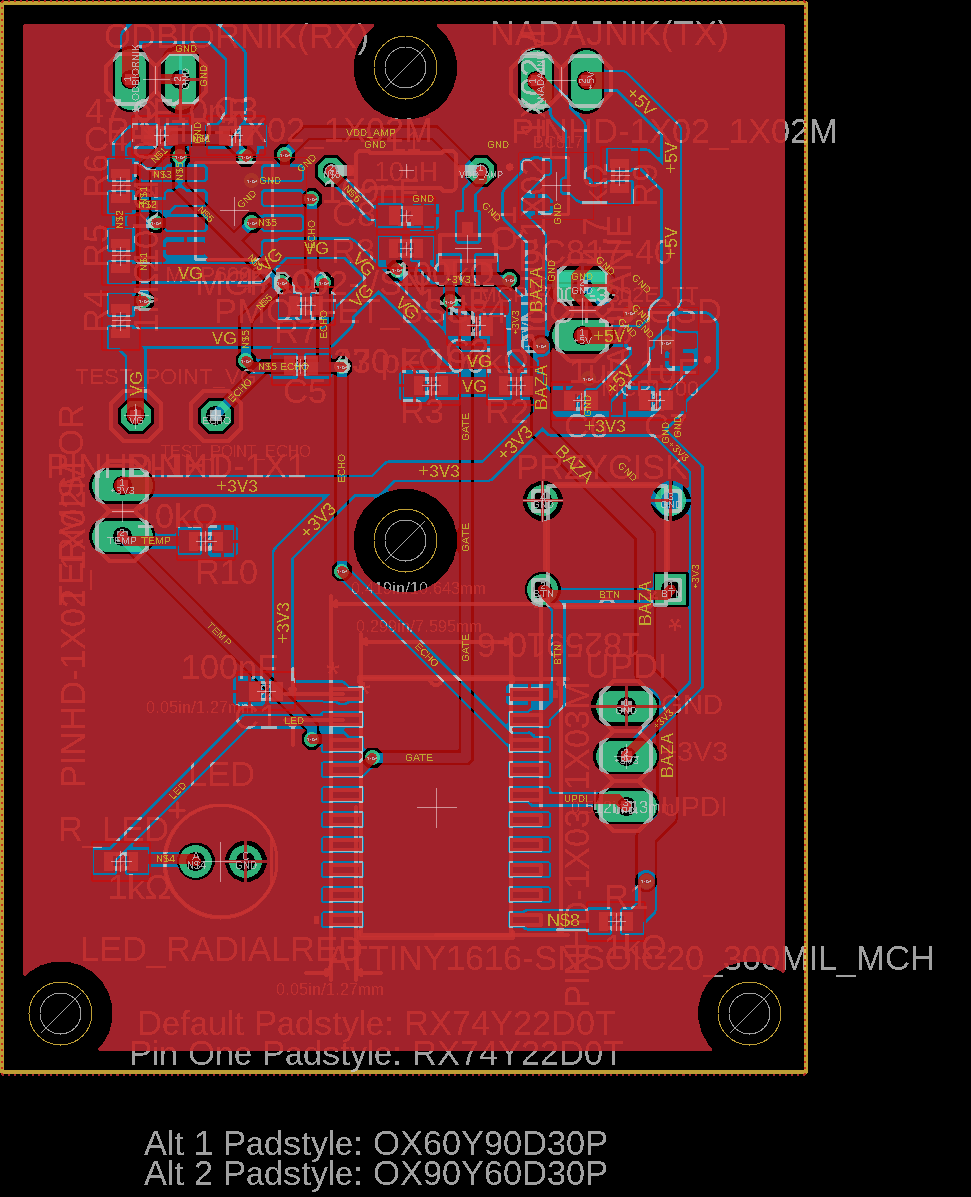
\includegraphics[width=0.7\textwidth]{pcb_top.png}
    \caption{Layout PCB --- widok z~góry (warstwa TOP)}
    \label{fig:pcb_top}
\end{figure}

Płytka drukowana zaprojektowana została w~programie EAGLE (Autodesk) jako
dwustronna (2-layer) o~wymiarach ${\sim}49 \times 36$~\si{\milli\metre}.

\subsection{Założenia projektowe PCB}

\begin{enumerate}[nosep]
    \item \textbf{Separacja analogowa/cyfrowa} --- sekcja wzmacniacza (MCP6002)
          umieszczona w~lewej części płytki, mikrokontroler w~prawej, z~minimalną
          liczbą skrzyżowań tras sygnałowych.
    \item \textbf{Ground plane} --- warstwa BOTTOM wykorzystana jako ciągła
          warstwa masy (ground plane), zapewniająca niską impedancję powrotną
          dla sygnałów analogowych i~redukcję sprzężeń EMI.
    \item \textbf{Kondensatory odsprzęgające} --- C1 (\SI{100}{\nano\farad})
          umieszczony bezpośrednio przy pinach VDD/GND ATtiny1616 (odległość
          $< \SI{3}{\milli\metre}$); C8 (\SI{100}{\nano\farad}) przy MCP6002.
    \item \textbf{Ścieżki sygnałowe} --- sygnał echa (ECHO) prowadzony
          możliwie krótką trasą od headera ODBIORNIK(RX) do wejścia MCP6002,
          następnie do pinu ADC mikrokontrolera.
    \item \textbf{Punkty testowe} --- TEST\_POINT\_ECHO i~TEST\_POINT\_VG
          (goldpiny 1x1) umożliwiają podłączenie oscyloskopu w~fazie debugowania.
    \item \textbf{Otwory montażowe} --- cztery otwory $\varnothing\SI{3,2}{\milli\metre}$
          w~narożnikach płytki umożliwiają mocowanie do obudowy lub podstawki.
\end{enumerate}

\subsection{Klasy tras i~reguły DRC}

\begin{table}[H]
    \centering
    \caption{Parametry ścieżek PCB}
    \label{tab:pcb_rules}
    \begin{tabular}{lr}
        \toprule
        \textbf{Parametr} & \textbf{Wartość} \\
        \midrule
        Szerokość ścieżki sygnałowej & \SI{0,254}{\milli\metre} (10\,mil) \\
        Szerokość ścieżki zasilania & \SI{0,508}{\milli\metre} (20\,mil) \\
        Prześwit minimalny & \SI{0,2}{\milli\metre} (8\,mil) \\
        Via drill & \SI{0,3}{\milli\metre} \\
        Via annular ring & \SI{0,15}{\milli\metre} \\
        Warstwa miedzi & \SI{35}{\micro\metre} (1\,oz) \\
        \bottomrule
    \end{tabular}
\end{table}


% ══════════════════════════════════════════════════════════════
% SEKCJA 5: ALGORYTM OPROGRAMOWANIA
% ══════════════════════════════════════════════════════════════
\clearpage
\section{Algorytm oprogramowania}
\label{sec:algorytm}

\subsection{Architektura oprogramowania}

Program mikrokontrolera został zaprojektowany w~języku C (AVR-GCC) z~podziałem
na moduły:

\begin{table}[H]
    \centering
    \caption{Moduły oprogramowania}
    \label{tab:moduly_sw}
    \begin{tabular}{lll}
        \toprule
        \textbf{Moduł} & \textbf{Plik} & \textbf{Funkcja} \\
        \midrule
        main & \texttt{main.c} & Pętla główna, inicjalizacja \\
        us\_driver & \texttt{us\_driver.c/h} & Generacja burstu, detekcja echa \\
        phase\_meas & \texttt{phase\_meas.c/h} & Algorytm Goertzela, obliczenie fazy \\
        temp\_comp & \texttt{temp\_comp.c/h} & Odczyt NTC, kompensacja $v(T)$ \\
        filter & \texttt{filter.c/h} & Filtr medianowy, uśrednianie \\
        uart & \texttt{uart.c/h} & Komunikacja USART \\
        power & \texttt{power.c/h} & Zarządzanie trybami uśpienia \\
        \bottomrule
    \end{tabular}
\end{table}

\subsection{Diagram przepływu}

\noindent Poniższy diagram przedstawia pełny cykl pomiarowy --- od inicjalizacji,
przez akwizycję i~przetwarzanie sygnału, po transmisję wyniku i~uśpienie mikrokontrolera.

\begin{figure}[H]
    \centering
    \begin{tikzpicture}[
        node distance=0.6cm,
        startstop/.style={rectangle, rounded corners, draw, fill=NavyBlue!15,
                          text width=4.5cm, align=center, minimum height=0.55cm, font=\footnotesize},
        process/.style={rectangle, draw, fill=white,
                        text width=4.8cm, align=center, minimum height=0.55cm, font=\footnotesize},
        decision/.style={diamond, draw, fill=orange!15,
                         text width=2.2cm, align=center, aspect=2.2, font=\footnotesize},
        io/.style={trapezium, draw, fill=Maroon!10, trapezium left angle=70,
                   trapezium right angle=110, text width=3.5cm, align=center,
                   minimum height=0.55cm, font=\footnotesize},
        arrow/.style={->, >=Stealth, semithick}
    ]
        \node[startstop] (init) {Inicjalizacja CLK, TCA0,\\TCB0, ADC0, USART};
        \node[process, below=of init] (temp) {Odczyt NTC (ADC, 4$\times$ oversample)\\$T \to v(T)$};
        \node[process, below=of temp] (burst) {TCA0: Nadaj burst\\$N=8$ cykli @ 40\,kHz};
        \node[process, below=of burst] (tof) {TCB0: Czekaj na echo\\$t_{ToF} \to D_{coarse}$};
        \node[decision, below=0.8cm of tof] (echo_ok) {Echo\\wykryte?};
        \node[process, right=1.5cm of echo_ok, font=\footnotesize] (err) {Błąd: brak echa};
        \node[process, below=0.8cm of echo_ok] (adc_win) {Otwórz okno pomiarowe\\ADC: $K$ próbek echa};
        \node[process, below=of adc_win] (goertzel) {Algorytm Goertzela $\to \varphi$};
        \node[process, below=of goertzel] (fusion) {Fuzja: $D = n \cdot \lambda/2 + D_{fine}$};
        \node[decision, below=0.8cm of fusion] (med_ok) {Zebrano\\$M$ pomiarów?};
        \node[process, below=0.8cm of med_ok] (filter) {Filtr medianowy $\to D_{filtered}$};
        \node[io, below=of filter] (uart) {USART TX: ,,D=XXX.X mm''};
        \node[startstop, below=of uart] (sleep) {POWER-DOWN SLEEP\\RTC wakeup $\to T_{cycle}$};

        \draw[arrow] (init) -- (temp);
        \draw[arrow] (temp) -- (burst);
        \draw[arrow] (burst) -- (tof);
        \draw[arrow] (tof) -- (echo_ok);
        \draw[arrow] (echo_ok) -- node[right, font=\scriptsize] {TAK} (adc_win);
        \draw[arrow] (echo_ok) -- node[above, font=\scriptsize] {NIE} (err);
        \draw[arrow] (err.south) |- (sleep.east);
        \draw[arrow] (adc_win) -- (goertzel);
        \draw[arrow] (goertzel) -- (fusion);
        \draw[arrow] (fusion) -- (med_ok);
        \draw[arrow] (med_ok) -- node[right, font=\scriptsize] {TAK ($M=7$)} (filter);
        \draw[arrow] (med_ok.west) -- ++(-2,0) |- node[left, pos=0.25, font=\scriptsize] {NIE} (temp.west);
        \draw[arrow] (filter) -- (uart);
        \draw[arrow] (uart) -- (sleep);
        \draw[arrow] (sleep.west) -- ++(-2.8,0) |- (temp.west);
    \end{tikzpicture}
    \caption{Diagram przepływu programu mikrokontrolera. Każdy wynik końcowy
    jest medianą z~$M = 7$ pomiarów jednostkowych.}
    \label{fig:flowchart}
\end{figure}

\subsection{Algorytm Goertzela --- wyznaczanie fazy sygnału echa}
\label{sec:goertzel}

Do wyznaczenia fazy sygnału echa przy częstotliwości $f_0 = \SI{40}{\kilo\hertz}$
zastosowano \textbf{algorytm Goertzela} --- wydajną obliczeniowo wariant DFT
dla pojedynczej częstotliwości. W~porównaniu z~pełnym FFT, algorytm Goertzela
wymaga jedynie $O(N)$ operacji mnożenia i~dodawania oraz minimalnej ilości
pamięci (${\sim}3$ zmienne stanu), co czyni go idealnym dla ATtiny1616.

\subsubsection{Podstawy matematyczne}

Algorytm oblicza składową Fouriera sygnału $x[n]$ przy znormalizowanej
częstotliwości $k = N \cdot f_0 / f_s$, gdzie $N$ to liczba próbek,
$f_s$ to częstotliwość próbkowania.

Rekurencja Goertzela:
\begin{equation}
    s[n] = x[n] + 2\cos\!\left(\frac{2\pi k}{N}\right) \cdot s[n-1] - s[n-2]
    \label{eq:goertzel_recur}
\end{equation}

z~warunkami początkowymi $s[-1] = s[-2] = 0$.

Po przetworzeniu wszystkich $N$ próbek, składowa zespolona:
\begin{equation}
    X[k] = s[N-1] - e^{-j2\pi k/N} \cdot s[N-2]
    \label{eq:goertzel_result}
\end{equation}

Faza sygnału:
\begin{equation}
    \varphi = \arctan\!\left(\frac{\text{Im}(X[k])}{\text{Re}(X[k])}\right)
    = \text{atan2}\!\left(\text{Im}(X[k]),\, \text{Re}(X[k])\right)
    \label{eq:goertzel_phase}
\end{equation}

gdzie:
\begin{align}
    \text{Re}(X[k]) &= s[N-1] - s[N-2] \cdot \cos(2\pi k / N) \label{eq:re} \\
    \text{Im}(X[k]) &= s[N-2] \cdot \sin(2\pi k / N) \label{eq:im}
\end{align}

\subsubsection{Parametry implementacji}

\begin{table}[H]
    \centering
    \caption{Parametry algorytmu Goertzela w~projekcie}
    \label{tab:goertzel_params}
    \begin{tabular}{lrl}
        \toprule
        \textbf{Parametr} & \textbf{Wartość} & \textbf{Uzasadnienie} \\
        \midrule
        $f_s$ & \SI{160}{\kilo\hertz} & $4 \times f_0$, zapas Nyquist \\
        $N$ & 16 & 4 pełne cykle @ $f_0$ \\
        $k$ & 4 & $N \cdot f_0/f_s = 16 \cdot 40/160$ \\
        $\cos(2\pi k/N)$ & $\cos(\pi/2) = 0$ & Uproszczenie! \\
        Czas obliczeń & ${\sim}\SI{50}{\micro\second}$ & 16-bit arytmetyka stałoprzecinkowa \\
        Zużycie RAM & ${\sim}\SI{20}{\byte}$ & 3 zmienne int32 + bufor \\
        \bottomrule
    \end{tabular}
\end{table}

\textbf{Kluczowa optymalizacja:} Dla $k = 4$ i~$N = 16$ współczynnik
$\cos(2\pi k/N) = \cos(\pi/2) = 0$, co redukuje rekurencję Goertzela do:
\begin{equation}
    s[n] = x[n] - s[n-2]
    \label{eq:goertzel_simplified}
\end{equation}

\textit{Eliminuje to mnożenie z~pętli rekurencyjnej}, pozostawiając jedynie
odejmowanie i~dodawanie --- idealnie nadające się dla mikrokontrolera bez
sprzętowego mnożnika zmiennoprzecinkowego.

\subsubsection{Pseudokod}

\begin{lstlisting}[caption={Algorytm Goertzela --- uproszczony dla $k=4$, $N=16$},
                   label={lst:goertzel}]
// Probkowanie ADC w oknie pomiarowym (ISR ADC)
int16_t samples[16];  // 16 probek @ 160 kHz

// Algorytm Goertzela (k=4, N=16 => cos(2*pi*k/N) = 0)
int32_t s0 = 0, s1 = 0, s2 = 0;
for (uint8_t n = 0; n < 16; n++) {
    s0 = (int32_t)samples[n] - s2;  // cos=0 eliminuje mnozenie!
    s2 = s1;
    s1 = s0;
}

// Skladowe Re i Im (sin(pi/2) = 1, cos(pi/2) = 0)
int32_t re = s1;       // s[N-1] - s[N-2]*cos = s[N-1]
int32_t im = s2;       // s[N-2]*sin = s[N-2]

// Faza (atan2 w arytmetyce staloprzecinkowej)
int16_t phase_deg = atan2_fixed(im, re);  // wynik w 0.1 stopnia

// Odleglosc fine
int32_t d_fine_um = (int32_t)phase_deg * lambda_half_um / 3600;
\end{lstlisting}

\subsection{Filtracja wyników --- filtr medianowy}
\label{sec:filtr}

W~celu redukcji szumu pomiarowego i~eliminacji wartości odstających (outliers
spowodowanych np.\ odbiciami wielokrotnymi) zastosowano filtr medianowy
z~oknem $M = 7$ pomiarów.

Filtr medianowy jest odporny na impulsowe zakłócenia (w~odróżnieniu od średniej
arytmetycznej) i~nie wymaga znajomości rozkładu szumu. Algorytm sortowania
dla $M = 7$ realizowany jest metodą sieci sortujących (sorting network) o~stałej
liczbie porównań $C = 16$ i~zamian $S \leq 16$, co zajmuje ${\sim}\SI{15}{\micro\second}$.

Po filtracji medianowej stosowana jest opcjonalna \textbf{wykładnicza średnia
krocząca} (EMA) z~parametrem $\alpha = 0{,}3$:
\begin{equation}
    D_{EMA}[k] = \alpha \cdot D_{median}[k] + (1-\alpha) \cdot D_{EMA}[k-1]
    \label{eq:ema}
\end{equation}

co wygładza wynik przy zachowaniu szybkiej reakcji na zmiany odległości.

\subsection{Procedura kalibracji}
\label{sec:kalibracja}

Przed pierwszym użyciem urządzenie wykonuje jednorazową procedurę kalibracyjną
mającą na celu kompensację systematycznych błędów:

\begin{enumerate}[nosep]
    \item \textbf{Kalibracja offsetu ToF} --- pomiar przy znanej odległości
          referencyjnej (np.\ \SI{20}{\centi\metre}), wyznaczenie offsetu
          $t_{offset}$ wynikającego z~opóźnień elektroniki i~ring-downu nadajnika.
    \item \textbf{Kalibracja fazy} --- pomiar przy dwóch znanych odległościach
          różniących się o~$\lambda/2$, weryfikacja liniowości pomiaru fazowego.
    \item \textbf{Współczynnik korekcji wzmocnienia} --- opcjonalne dopasowanie
          krzywej $D_{measured} = a \cdot D_{raw} + b$ metodą najmniejszych
          kwadratów dla 3--5 punktów referencyjnych.
\end{enumerate}

Parametry kalibracyjne zapisywane są w~pamięci EEPROM ATtiny1616
(\SI{256}{\byte} dostępne).

\subsection{Komunikacja USART}
\label{sec:usart}

Wynik pomiaru transmitowany jest przez USART0 (pin PA1/TXD) w~formacie ASCII:

\begin{lstlisting}[caption={Format ramki wyjściowej USART}, label={lst:uart_frame}]
// Format: "D=XXX.X mm\r\n"
// Przyklad: "D=234.7 mm\r\n"
// Baudrate: 9600 bps (8N1)
// Odczyt: dowolny terminal szeregowy (PuTTY, screen, minicom)
// Podlaczenie: UPDI header pin 1 (TX) + GND
\end{lstlisting}

Transmisja jednej ramki (${\sim}16$ znaków @ 9600\,bps) trwa ${\sim}\SI{17}{\milli\second}$.
W~trybie oszczędnym USART jest wyłączany między transmisjami.


% ══════════════════════════════════════════════════════════════
% SEKCJA 6: BUDŻET KOSZTÓW
% ══════════════════════════════════════════════════════════════
\section{Budżet kosztów}
\label{sec:koszty}

\begin{table}[H]
    \centering
    \caption{Koszt elementów urządzenia (wg regulaminu i~cen brutto sklepów)}
    \label{tab:koszty}
    \begin{tabular}{llrrrl}
        \toprule
        \textbf{Element} & \textbf{Ozn.} & \textbf{Ilość} &
        \textbf{Cena/szt.} & \textbf{Suma} & \textbf{Źródło} \\
        \midrule
        \multicolumn{6}{l}{\textit{Elementy R, L, C, tranzystory i~diody małej mocy --- \SI{0,15}{PLN}/szt.\ (regulamin):}} \\
        \midrule
        Rezystory 0603 & R1--R10, R\_LED & 11 & 0,15 & 1,65 & regulamin \\
        Kondensatory 0603 & C1--C8 & 8 & 0,15 & 1,20 & regulamin \\
        Cewka \SI{10}{\micro\henry} & L1 & 1 & 0,15 & 0,15 & regulamin \\
        BC817-40 (NPN) & BC817 & 1 & 0,15 & 0,15 & regulamin \\
        LED czerwona & LED & 1 & 0,15 & 0,15 & regulamin \\
        \midrule
        \multicolumn{6}{l}{\textit{Wzmacniacze operacyjne --- \SI{1,00}{PLN}/szt.\ (regulamin):}} \\
        \midrule
        MCP6002-I/SN & MCP6002 & 1 & 1,00 & 1,00 & regulamin \\
        \midrule
        \multicolumn{6}{l}{\textit{PCB --- cena regulaminowa:}} \\
        \midrule
        Płytka drukowana & PCB & 1 & 15,00 & 15,00 & regulamin \\
        \midrule
        \multicolumn{6}{l}{\textit{Pozostałe elementy --- ceny brutto sklepów na terenie UE:}} \\
        \midrule
        ATtiny1616-SN & U1 & 1 & 8,50 & 8,50 &
            \href{https://www.tme.eu/pl/details/attiny1616-snr/mikrokontrolery-microchip-avr-8-bit/microchip-technology/}{TME} \\
        MCP1700T-3302E/TT & U2 & 1 & 1,63 & 1,63 &
            \href{https://www.tme.eu/pl/details/mcp1700t-3302e_tt/stabilizatory-ldo-nienastawne/microchip-technology/}{TME} \\
        Przycisk 1825910-6 & SW1 & 1 & 0,98 & 0,98 &
            \href{https://www.tme.eu/pl/details/1825910-6/przelaczniki-tact/te-connectivity/}{TME} \\
        Goldpiny 1x02 & --- & 4 & 0,30 & 1,20 &
            \href{https://www.tme.eu/pl/}{TME} \\
        Goldpiny 1x03 & UPDI & 1 & 0,35 & 0,35 &
            \href{https://www.tme.eu/pl/}{TME} \\
        Goldpiny 1x01 & TP & 2 & 0,15 & 0,30 &
            \href{https://www.tme.eu/pl/}{TME} \\
        Nadajnik US 40\,kHz & TX & 1 & 3,50 & 3,50 &
            \href{https://www.tme.eu/pl/}{TME} \\
        Odbiornik US 40\,kHz & RX & 1 & 3,50 & 3,50 &
            \href{https://www.tme.eu/pl/}{TME} \\
        Termistor NTC 10\,k$\Omega$ & NTC & 1 & 0,90 & 0,90 &
            \href{https://www.tme.eu/pl/}{TME} \\
        \midrule
        \multicolumn{4}{r}{\textbf{RAZEM (koszt brutto):}} & \textbf{40,16} & PLN \\
        \bottomrule
    \end{tabular}
\end{table}

Punkty za cenę elementów:
\begin{equation}
    P_{cena} = \min\!\left(50,\; \frac{50 \times 50}{40{,}16}\right)
    = \min(50;\; 62{,}3) = \textbf{50~pkt~(max)}
    \label{eq:pkt_cena}
\end{equation}


% ══════════════════════════════════════════════════════════════
% SEKCJA 7: BUDŻET MOCY
% ══════════════════════════════════════════════════════════════
\section{Budżet mocy}
\label{sec:moc}

\subsection{Prąd pobierany przez poszczególne elementy}

\begin{table}[H]
    \centering
    \caption{Szczegółowy budżet prądowy (dane z~kart katalogowych)}
    \label{tab:moc_detail}
    \begin{tabular}{lrrrr}
        \toprule
        \textbf{Element} & \textbf{$I_{active}$} & \textbf{$I_{sleep}$}
            & \textbf{$t_{active}$} & \textbf{Źródło danych} \\
        \midrule
        ATtiny1616 @ 20\,MHz
            & \SI{10}{\milli\ampere}
            & \SI{0,1}{\micro\ampere}
            & \SI{5}{\milli\second}
            & DS, Fig.~33-9 \\
        MCP6002 (oba kanały)
            & \SI{100}{\micro\ampere}
            & \SI{100}{\micro\ampere}
            & ciągły
            & DS, Tab.~1.1 \\
        MCP1700 ($I_q$)
            & \SI{1,6}{\micro\ampere}
            & \SI{1,6}{\micro\ampere}
            & ciągły
            & DS, Tab.~1 \\
        Nadajnik US (burst)
            & \SI{20}{\milli\ampere}
            & \SI{0}{\micro\ampere}
            & \SI{0,2}{\milli\second}
            & estymacja \\
        LED (puls)
            & \SI{3,3}{\milli\ampere}
            & \SI{0}{\micro\ampere}
            & \SI{1}{\milli\second}
            & $R_{LED} = \SI{1}{\kilo\ohm}$ \\
        \bottomrule
    \end{tabular}
\end{table}

\subsection{Scenariusze pracy}

\subsubsection{Scenariusz 1: Ciągły pomiar (bez uśpienia)}

Przy ciągłym działaniu wszystkich elementów:
\begin{equation}
    I_{avg,1} = 10 + 0{,}1 + 0{,}002 + 20 \cdot 0{,}04 + 3{,}3 \cdot 0{,}2 \approx \SI{11,6}{\milli\ampere}
\end{equation}
\begin{equation}
    P_{in,1} = I_{avg,1} \cdot V_{in} = 11{,}6 \cdot 5{,}0 = \SI{58}{\milli\watt}, \quad
    P_{pkt,1} = 100/58 \approx \textbf{1,7~pkt}
\end{equation}

\subsubsection{Scenariusz 2: Pomiar okresowy ze sleep mode (planowany)}

Cykl pomiarowy: $T_{cycle} = \SI{100}{\milli\second}$, czas aktywny
$t_{active} = \SI{5}{\milli\second}$ (burst + ToF + ADC + Goertzel + UART),
czas uśpienia $t_{sleep} = \SI{95}{\milli\second}$.

Średni prąd mikrokontrolera:
\begin{equation}
    I_{MCU,avg} = \frac{t_{active} \cdot I_{active} + t_{sleep} \cdot I_{sleep}}{T_{cycle}}
    = \frac{5 \cdot 10000 + 95 \cdot 0{,}1}{100} \approx \SI{500}{\micro\ampere}
    \label{eq:imcu_avg}
\end{equation}

Średni prąd całkowity (@ \SI{3,3}{\volt}):
\begin{equation}
    I_{avg,2} = 500 + 100 + 1{,}6 + 20000 \cdot \frac{0{,}2}{100} + 3300 \cdot \frac{1}{100}
    \approx \SI{675}{\micro\ampere}
\end{equation}

Moc pobierana z~zasilania \SI{5}{\volt}:
\begin{equation}
    P_{in,2} = \frac{I_{avg,2} \cdot V_{3,3}}{\eta_{LDO}} = \frac{0{,}675 \cdot 3{,}3}{0{,}66}
    \approx \SI{3,4}{\milli\watt}, \quad
    P_{pkt,2} = 100/3{,}4 \approx \textbf{29~pkt}
    \label{eq:moc_scen2}
\end{equation}

\subsubsection{Scenariusz 3: Agresywna optymalizacja (cel)}

Dodatkowe optymalizacje planowane w~Etapie~2:
\begin{itemize}[nosep]
    \item Wyłączanie MCP6002 przez odcięcie zasilania pinem GPIO + P-MOSFET
          ($I_{sleep,opamp} = \SI{0}{\micro\ampere}$)
    \item Redukcja $T_{cycle}$ do \SI{200}{\milli\second} (pomiar co 5/s)
    \item Taktowanie MCU na \SI{5}{\mega\hertz} w~fazie obliczeń
          ($I_{active} \approx \SI{3}{\milli\ampere}$)
    \item Wyłączanie LED (wynik tylko przez UART)
\end{itemize}

Szacowany średni prąd:
\begin{equation}
    I_{avg,3} \approx \SI{200}{\micro\ampere}, \quad
    P_{in,3} \approx \SI{1,0}{\milli\watt}, \quad
    P_{pkt,3} = \min(50, 100/1{,}0) = \textbf{50~pkt~(max)}
    \label{eq:moc_scen3}
\end{equation}


% ══════════════════════════════════════════════════════════════
% SEKCJA 8: ANALIZA BŁĘDÓW
% ══════════════════════════════════════════════════════════════
\section{Analiza błędów i~niepewność pomiaru}
\label{sec:bledy}

\subsection{Budżet niepewności}

\begin{table}[H]
    \centering
    \caption{Szczegółowy budżet niepewności pomiaru @ $D = \SI{30}{\centi\metre}$, $T = \SI{20}{\celsius}$}
    \label{tab:bledy}
    \begin{tabularx}{\textwidth}{lrrX}
        \toprule
        \textbf{Źródło} & \textbf{$\sigma$ [\si{\milli\metre}]} & \textbf{Typ}
            & \textbf{Kompensacja / redukcja} \\
        \midrule
        Szum ADC (10-bit, 1\,LSB)
            & 0,10
            & Losowy
            & Oversampling $4\times$ ($\to \sigma/2$), Goertzel filtruje szum poza $f_0$ \\
        Niepewność pomiaru fazy
            & 0,15
            & Losowy
            & Uśrednianie z~$M=7$ pomiarów ($\to \sigma/\sqrt{7}$) \\
        Kompensacja temperatury (resztkowa)
            & 0,05
            & Systematyczny
            & Termistor NTC z~oversamplingiem ($\Delta T < \SI{0,1}{\kelvin}$) \\
        Jitter zegara ($\pm\SI{2}{\percent}$ int.\ osc.)
            & 0,12
            & Losowy
            & Kalibracja oscylatora, pomiar różnicowy \\
        Kąt padania wiązki US
            & 0,20
            & Systematyczny
            & Mechaniczne ustawienie, karton $20\times20$\,cm redukuje wrażliwość \\
        Odbicia wielokrotne (multipath)
            & 0,30
            & Losowy
            & Filtr medianowy eliminuje outliers, bramkowanie czasowe \\
        Ring-down nadajnika (bliskie pole)
            & 0,15
            & Systematyczny
            & Kalibracja offsetu ToF, $D_{min} = \SI{10}{\centi\metre}$ (\SI{0,6}{\milli\second} --- wystarczający czas wygaszenia) \\
        Rozrzut $f_0$ przetworników
            & 0,10
            & Systematyczny
            & Jednorazowa kalibracja, zapis w~EEPROM \\
        \bottomrule
    \end{tabularx}
\end{table}

\subsection{Szacowany RMSE}

Zakładając nieskorelowanie poszczególnych źródeł błędu, sumaryczna
niepewność standardowa (przed filtracją):
\begin{equation}
    \sigma_{total} = \sqrt{\sum_i \sigma_i^2}
    = \sqrt{0{,}10^2 + 0{,}15^2 + 0{,}05^2 + 0{,}12^2 + 0{,}20^2 + 0{,}30^2 + 0{,}15^2 + 0{,}10^2}
    \approx \SI{0,48}{\milli\metre}
    \label{eq:sigma_total}
\end{equation}

Po filtracji medianowej ($M = 7$) i~EMA ($\alpha = 0{,}3$), efektywna
redukcja szumu losowego o~czynnik ${\sim}2{,}5$:
\begin{equation}
    \boxed{RMSE_{est} \approx \SI{0,3}{\milli\metre} \text{ -- } \SI{0,8}{\milli\metre}}
    \label{eq:rmse_final}
\end{equation}

Dolna granica (0,3\,mm) odpowiada idealnemu scenariuszowi z~dobrze
skalibrowanym urządzeniem; górna (0,8\,mm) --- warunkom niekontrolowanym
z~odbiciami. W~obu przypadkach wynik jest znacząco lepszy niż osiągalny
metodą prostego ToF (${\sim}\SI{3}{\milli\metre}$).


% ══════════════════════════════════════════════════════════════
% SEKCJA 9: PODSUMOWANIE
% ══════════════════════════════════════════════════════════════
\section{Podsumowanie i~planowane optymalizacje}
\label{sec:podsumowanie}

\subsection{Szacowana punktacja}

\begin{table}[H]
    \centering
    \caption{Podsumowanie szacowanej punktacji}
    \label{tab:punktacja}
    \begin{tabular}{lrrr}
        \toprule
        \textbf{Kryterium} & \textbf{Max} & \textbf{Pesymist.} & \textbf{Optymist.} \\
        \midrule
        Błąd RMSE         & 100 & 70  & 95 \\
        Średni pobór mocy & 50  & 29  & 50 \\
        Koszt elementów   & 50  & 50  & 50 \\
        Jakość projektu   & 100 & 65  & 90 \\
        \midrule
        \textbf{RAZEM}    & \textbf{300} & \textbf{214} & \textbf{285} \\
        \bottomrule
    \end{tabular}
\end{table}

\subsection{Planowane optymalizacje na Etap 2}

Na etapie budowy prototypu planowane są następujące działania optymalizacyjne:

\begin{enumerate}[nosep]
    \item \textbf{Optymalizacja toru analogowego} --- eksperymentalny dobór
          wartości C4 i~C5 w~celu maksymalizacji wzmocnienia przy $f_0$ (patrz
          sekcja \ref{sec:tor_rx}). Cel: $|A_{total}| \geq 10$.
    \item \textbf{Agresywne zarządzanie mocą} --- wyłączanie MCP6002 przez
          P-MOSFET, redukcja częstotliwości zegara MCU w~fazie obliczeń.
          Cel: $P_{avg} < \SI{2}{\milli\watt}$.
    \item \textbf{Kalibracja wielopunktowa} --- pomiary w~5--10 punktach
          referencyjnych, dopasowanie krzywej korekcyjnej (wielomian 2.~stopnia
          lub look-up table z~interpolacją liniową). Zapis w~EEPROM.
    \item \textbf{Push-pull sterowanie nadajnika} --- wykorzystanie dwóch pinów
          GPIO w~przeciwfazie do podwojenia amplitudy sygnału TX (poprawa SNR
          o~\SI{6}{\deci\bel}).
    \item \textbf{Automatyczna regulacja wzmocnienia (AGC)} --- wykorzystanie
          DAC0 ATtiny1616 do dynamicznej regulacji offsetu/wzmocnienia toru
          analogowego w~zależności od zmierzonej odległości.
    \item \textbf{Projekt obudowy} --- druk 3D obudowy z~precyzyjnym mocowaniem
          przetworników US (kąt, odstęp), minimalizujący wpływ geometrii na pomiar.
\end{enumerate}

\subsection{Wnioski}

Zaprojektowany miernik odległości wykorzystuje hybrydową metodę Pulse-Phase
Ranging, która łączy prostotę i~niski koszt ultradźwiękowego pomiaru ToF
z~sub-milimetrową rozdzielczością pomiaru fazowego. Kluczowymi zaletami
rozwiązania są:

\begin{itemize}[nosep]
    \item Teoretyczny RMSE poniżej \SI{1}{\milli\metre} dzięki algorytmowi Goertzela.
    \item Koszt elementów ${\sim}\SI{40}{PLN}$ --- maksymalna punktacja (50\,pkt).
    \item Potencjał redukcji poboru mocy do ${\sim}\SI{1}{\milli\watt}$ (50\,pkt).
    \item Kompensacja temperatury eliminująca dominujące źródło błędu systematycznego.
    \item Modułowa architektura oprogramowania ułatwiająca dalszą optymalizację.
\end{itemize}

Projekt demonstruje świadome podejmowanie decyzji inżynierskich na każdym
etapie --- od wyboru metody pomiarowej, przez dobór komponentów i~topologię
PCB, po algorytm przetwarzania sygnałów i~strategię zarządzania energią.
Autor jest przekonany, że zaproponowane rozwiązanie stanowi solidną podstawę
do budowy prototypu w~Etapie~2 konkursu.

\end{document}